% IT5006 Phase 2 final report, version 4: teammates' v1, corrected and condensed with v3 content.
% Run phase2_final/reports/phase2_final_evidence.py after updating saved results; it refreshes
% only the marked number and figure blocks below. This file compiles standalone.
\documentclass[12pt,a4paper]{article}
\usepackage[margin=0.8in]{geometry}
\usepackage[T1]{fontenc}
\usepackage{lmodern}
\usepackage{microtype}
\usepackage{booktabs}
\usepackage{array}
\usepackage{graphicx}
\usepackage{tikz}
\usepackage{float}
\usepackage{pgfplots}
\pgfplotsset{compat=1.16}
\usepackage{hyperref}
\hypersetup{colorlinks=true,linkcolor=blue,urlcolor=blue}
\setlength{\parindent}{0pt}
\setlength{\parskip}{0.4em}
\renewcommand{\arraystretch}{1.1}
% BEGIN GENERATED numbers -- refreshed by phase2_final_evidence.py
% Generated by reports/phase2_final_evidence.py: do not edit by hand.
\newcommand{\ActShare}{13}
\newcommand{\AllOrders}{96{,}272}
\newcommand{\AugModelNotPast}{79}
\newcommand{\AugRuleNotPast}{113}
\newcommand{\BadReviewLate}{62}
\newcommand{\BadReviewOnTime}{9}
\newcommand{\BadReviewRatio}{6.7}
\newcommand{\BenefitRatio}{5}
\newcommand{\BlackFridayLate}{12}
\newcommand{\BreakEvenRandomTest}{29}
\newcommand{\BreakEvenTest}{6.5}
\newcommand{\BreakEvenVal}{3.1}
\newcommand{\BusyGainMax}{28}
\newcommand{\BusyGainMin}{20}
\newcommand{\BusyRateMax}{21}
\newcommand{\BusyRateMin}{10}
\newcommand{\CalmGainMax}{25}
\newcommand{\CalmGainMin}{14}
\newcommand{\CalmRateMax}{5}
\newcommand{\CalmWindows}{W1 and W3}
\newcommand{\CarrierMean}{9.3}
\newcommand{\CarrierShare}{85}
\newcommand{\CheckoutBestMAE}{5.78}
\newcommand{\CheckoutBestName}{forest\_leaf20}
\newcommand{\CheckoutBestRMSE}{9.34}
\newcommand{\CheckoutBestRSq}{0.176}
\newcommand{\CheckoutImpAName}{numeric\_\_promised\_days}
\newcommand{\CheckoutImpAVal}{1.780}
\newcommand{\CheckoutImpBName}{logged\_\_distance\_km}
\newcommand{\CheckoutImpBVal}{1.111}
\newcommand{\CheckoutImpCName}{numeric\_\_route\_typical\_days}
\newcommand{\CheckoutImpCVal}{0.882}
\newcommand{\CheckoutImpKind}{coefficient (mean $|$weight$|$ over windows, numeric and engineered inputs; one-hot state/category dummies excluded from this ranking)}
\newcommand{\CheckoutMeanMAE}{7.21}
\newcommand{\CheckoutMeanRMSE}{10.67}
\newcommand{\CheckoutMeanRSq}{-0.078}
\newcommand{\CheckoutPR}{0.213}
\newcommand{\CheckoutRandTestMAE}{5.04}
\newcommand{\CheckoutRandTestRSq}{0.276}
\newcommand{\CheckoutRandValRSq}{0.259}
\newcommand{\CheckoutSelGap}{0.026}
\newcommand{\CheckoutSelGapSE}{0.028}
\newcommand{\CheckoutSelMAE}{5.81}
\newcommand{\CheckoutSelName}{ridge\_100}
\newcommand{\CheckoutSelRMSE}{9.40}
\newcommand{\CheckoutSelRSq}{0.167}
\newcommand{\CheckoutTestBias}{3.65}
\newcommand{\CheckoutTestMAE}{5.00}
\newcommand{\CheckoutTestRMSE}{6.41}
\newcommand{\CheckoutTestRSq}{-0.175}
\newcommand{\ClsBestName}{logistic\_c0.01}
\newcommand{\ClsCheckoutSelName}{logistic\_c0.01}
\newcommand{\ClsDefaultPR}{0.359}
\newcommand{\ClsNetBenefit}{-0.029}
\newcommand{\ClsPlainName}{logistic\_unregularized}
\newcommand{\ClsPlainPR}{0.354}
\newcommand{\ClsSelGap}{0.000}
\newcommand{\ClsSelGapSE}{0.000}
\newcommand{\ClsSelName}{logistic\_c0.01}
\newcommand{\ClsTestFone}{0.24}
\newcommand{\ClsTestLate}{3.5}
\newcommand{\ClsTestMCC}{0.25}
\newcommand{\ClsTestPR}{0.48}
\newcommand{\ClsTestPrec}{15.5}
\newcommand{\ClsTestROC}{0.85}
\newcommand{\ClsTestRec}{58}
\newcommand{\CohortOrders}{96{,}272}
\newcommand{\DisruptLateShare}{72}
\newcommand{\EtaTestOrders}{19{,}230}
\newcommand{\EtaTrainOrders}{75{,}039}
\newcommand{\ExcludedOrders}{198}
\newcommand{\FebMarLate}{17}
\newcommand{\FullDailyActiveDays}{81}
\newcommand{\FullDailyBeforePromise}{208}
\newcommand{\FullDailyCaught}{414}
\newcommand{\FullDailyCaughtOpen}{413}
\newcommand{\FullDailyCaughtPerDay}{5}
\newcommand{\FullDailyExpiredCaught}{206}
\newcommand{\FullDailyFlagged}{2{,}584}
\newcommand{\FullDailyLate}{705}
\newcommand{\FullDailyMedianFlagged}{36}
\newcommand{\FullDailyOrders}{19{,}534}
\newcommand{\FullDailyPninetyFlagged}{52}
\newcommand{\FullDailyPrecision}{16.0}
\newcommand{\FullDailyRecall}{58.7}
\newcommand{\FullDailyRecallRound}{59}
\newcommand{\GainFiveModel}{46}
\newcommand{\GainOneModel}{20}
\newcommand{\GainTenModel}{54}
\newcommand{\GainTwentyModel}{66}
\newcommand{\HandoverBestMAE}{5.10}
\newcommand{\HandoverBestName}{ridge\_100}
\newcommand{\HandoverBestRMSE}{8.41}
\newcommand{\HandoverBestRSq}{0.338}
\newcommand{\HandoverImpAName}{numeric\_\_handover\_days}
\newcommand{\HandoverImpAVal}{3.436}
\newcommand{\HandoverImpBName}{logged\_\_distance\_km}
\newcommand{\HandoverImpBVal}{1.218}
\newcommand{\HandoverImpCName}{numeric\_\_promise\_slack}
\newcommand{\HandoverImpCVal}{1.003}
\newcommand{\HandoverImpKind}{coefficient (mean $|$weight$|$ over windows, numeric and engineered inputs; one-hot state/category dummies excluded from this ranking)}
\newcommand{\HandoverMeanMAE}{7.21}
\newcommand{\HandoverMeanRMSE}{10.67}
\newcommand{\HandoverMeanRSq}{-0.078}
\newcommand{\HandoverRandTestMAE}{4.34}
\newcommand{\HandoverRandTestRSq}{0.411}
\newcommand{\HandoverRandValRSq}{0.386}
\newcommand{\HandoverRuleMAE}{5.30}
\newcommand{\HandoverRuleRSq}{0.337}
\newcommand{\HandoverSelGap}{0.000}
\newcommand{\HandoverSelGapSE}{0.000}
\newcommand{\HandoverSelMAE}{5.10}
\newcommand{\HandoverSelName}{ridge\_100}
\newcommand{\HandoverSelRMSE}{8.41}
\newcommand{\HandoverSelRSq}{0.338}
\newcommand{\HandoverTestBias}{2.87}
\newcommand{\HandoverTestMAE}{3.97}
\newcommand{\HandoverTestRMSE}{5.44}
\newcommand{\HandoverTestRSq}{0.154}
\newcommand{\ImpADrop}{0.088}
\newcommand{\ImpAName}{slack\_shortfall}
\newcommand{\ImpBDrop}{0.046}
\newcommand{\ImpBName}{handover\_days}
\newcommand{\ImpCDrop}{0.039}
\newcommand{\ImpCName}{remaining\_slack}
\newcommand{\ImpDDrop}{0.016}
\newcommand{\ImpDName}{distance\_km}
\newcommand{\ImpEDrop}{0.016}
\newcommand{\ImpEName}{route\_typical\_days}
\newcommand{\ImpFDrop}{0.014}
\newcommand{\ImpFName}{promised\_days}
\newcommand{\JunModelNotPast}{30}
\newcommand{\JunRuleNotPast}{30}
\newcommand{\LadderCheckoutMAE}{5.81}
\newcommand{\LadderCheckoutMinRSq}{0.060}
\newcommand{\LadderCheckoutRSq}{0.167}
\newcommand{\LadderElapsedMAE}{5.11}
\newcommand{\LadderElapsedMinRSq}{0.222}
\newcommand{\LadderElapsedRSq}{0.335}
\newcommand{\LadderHandoverMAE}{5.10}
\newcommand{\LadderHandoverMinRSq}{0.227}
\newcommand{\LadderHandoverRSq}{0.338}
\newcommand{\LadderTransitMAE}{5.68}
\newcommand{\LadderTransitMinRSq}{0.078}
\newcommand{\LadderTransitRSq}{0.214}
\newcommand{\LaterLift}{4.4}
\newcommand{\LaterLossPct}{9}
\newcommand{\LaterModelCaught}{387}
\newcommand{\LaterRuleCaught}{424}
\newcommand{\NormalLate}{4}
\newcommand{\OosGainPct}{12}
\newcommand{\OosModelCaught}{1{,}384}
\newcommand{\OosRuleCaught}{1{,}241}
\newcommand{\OosWins}{3}
\newcommand{\PastPromiseLateRate}{99.4}
\newcommand{\PastPromiseTest}{29.5}
\newcommand{\PastPromiseVal}{4.1}
\newcommand{\PastPromiseWinMax}{12}
\newcommand{\PastPromiseWinMin}{1}
\newcommand{\PrecFiveModel}{32}
\newcommand{\PrecOneModel}{70}
\newcommand{\PrecTenModel}{19}
\newcommand{\PrecTwentyModel}{12}
\newcommand{\PromAug}{15.2}
\newcommand{\PromJul}{19.7}
\newcommand{\PromJun}{27.8}
\newcommand{\PromSpanMax}{28}
\newcommand{\PromSpanMin}{22}
\newcommand{\RatedOrders}{95{,}627}
\newcommand{\RepeatAfterLate}{2.5}
\newcommand{\RepeatAfterOnTime}{3.0}
\newcommand{\RepeatShare}{3.0}
\newcommand{\RuleGapHigh}{0.062}
\newcommand{\RuleGapLow}{0.047}
\newcommand{\RuleGapPR}{0.054}
\newcommand{\RuleNetBenefit}{-0.020}
\newcommand{\RuleRecallTen}{59}
\newcommand{\RuleTestFone}{0.27}
\newcommand{\RuleTestPR}{0.52}
\newcommand{\RuleTestPrec}{16.9}
\newcommand{\RuleTestROC}{0.88}
\newcommand{\RuleTestRec}{63}
\newcommand{\RuleValPR}{0.328}
\newcommand{\ShapeBeatsRuleWindows}{5}
\newcommand{\ShapeRecallWith}{54}
\newcommand{\ShapeRecallWithout}{41}
\newcommand{\ShapeTestWith}{0.48}
\newcommand{\ShapeTestWithout}{0.23}
\newcommand{\ShapeValWith}{0.382}
\newcommand{\ShapeValWithout}{0.367}
\newcommand{\ShapeWinsWindows}{5}
\newcommand{\ShortCut}{14.5}
\newcommand{\ShortShareAug}{56}
\newcommand{\ShortTestPRModel}{0.146}
\newcommand{\ShortTestPRRule}{0.195}
\newcommand{\ShortValLateMax}{53}
\newcommand{\ShortValLateMin}{3}
\newcommand{\ShortValModelWins}{3}
\newcommand{\TestAugActed}{820}
\newcommand{\TestAugCaught}{234}
\newcommand{\TestAugLateCount}{393}
\newcommand{\TestAugOrders}{6{,}306}
\newcommand{\TestJulActed}{796}
\newcommand{\TestJulCaught}{119}
\newcommand{\TestJulLateCount}{207}
\newcommand{\TestJulOrders}{6{,}119}
\newcommand{\TestJunActed}{787}
\newcommand{\TestJunCaught}{33}
\newcommand{\TestJunLateCount}{70}
\newcommand{\TestJunOrders}{6{,}050}
\newcommand{\TestMayActed}{99}
\newcommand{\TestMayCaught}{1}
\newcommand{\TestMayLateCount}{2}
\newcommand{\TestMayOrders}{755}
\newcommand{\TestOrders}{19{,}230}
\newcommand{\TotalMean}{12.6}
\newcommand{\TrainPromised}{24.3}
\newcommand{\UniqueCustomers}{93{,}159}
\newcommand{\ValBestPR}{0.382}
\newcommand{\ValGainMax}{28}
\newcommand{\ValGainMin}{14}
\newcommand{\ValNetBenefit}{0.077}
\newcommand{\ValSelPR}{0.382}
\newcommand{\ValSelROC}{0.774}
\newcommand{\ValSelRecallTen}{36}
\newcommand{\WFiveModelCaught}{533}
\newcommand{\WFiveRuleCaught}{443}
\newcommand{\WTwoModelCaught}{401}
\newcommand{\WTwoRuleCaught}{313}
\newcommand{\WalkMaxGap}{0.003}
\newcommand{\WalkSame}{3}
% END GENERATED numbers

\begin{document}
\begin{titlepage}
\centering
\vspace*{0.8cm}
\IfFileExists{NUS_logo_full-horizontal.jpg}{%
  
\includegraphics[width=0.6\textwidth]{NUS_logo_full-horizontal.jpg}\par
}{%
  \IfFileExists{reports/NUS_logo_full-horizontal.jpg}{%
    \includegraphics[width=0.6\textwidth]{reports/NUS_logo_full-horizontal.jpg}\par
  }{%
    {\Huge\bfseries NUS\par}
    \vspace{0.2cm}
    {\large National University of Singapore\par}
    \vspace{1.8cm}
  }%
}
\vspace{1.6cm}
{\LARGE\bfseries Keeping Delivery Promises at Olist\par}
\vspace{0.4cm}
{\large Two-stage Delivery-time Estimation and Late-order Prioritisation at Carrier Handover\par}
\vspace{1.3cm}
{\large\bfseries IT5006 Phase 2\par}
\vspace{0.3cm}
{\large AY2026/27 Semester 1\par}
\vspace{1.4cm}
{\large\bfseries Group 6\par}
\vspace{0.6cm}
{\normalsize
CHAI WEI NI, WINNIE (A0172261M)\par
LE TRUNG HIEU (A0286973H)\par
LIANG ZIYAN (A0291506E)\par
LUM ZI YUAN JOSHUA (A0108499N)\par
SHAH PRATIK (A0211041H)\par
YUAN JIAYI (A0177893H)\par
}
\vfill
{\footnotesize Code and notebooks: \url{https://github.com/YuanJiayi/Team6_IT5006_Ecommerce_Analytics_AY2627Sem1}}\par
\vspace*{0.5cm}
\end{titlepage}

\section*{Executive Summary}
Late deliveries hurt Olist's reviews: \BadReviewLate{}\% of late orders receive a one- or two-star review, against \BadReviewOnTime{}\% of on-time orders. Our aim is to help the delivery operations team act on late orders early. When a seller hands a parcel to the carrier, two models help. The \textbf{classifier} ranks that day's parcels by their risk of missing the date the customer was promised. The \textbf{regression} estimates how many more days each delivery will take. Figure~\ref{fig:workflow} shows where both sit in an order's journey.

\begin{itemize}\setlength{\itemsep}{0pt}
\item \textbf{Delivery-time estimate.} Our chosen regression is a ridge regression ($\alpha=100$), selected on validation from four model families. At checkout it has an MAE of \CheckoutSelMAE{} days. Once the carrier has the parcel, we update the estimate using how long the order has already taken, and the MAE falls to \HandoverSelMAE{} days. The update is more accurate in every validation period, and it beats a simple rule of thumb, days so far plus the route's usual carrier time (MAE \HandoverRuleMAE{} days).
\item \textbf{Late warning.} Without a model, staff could rank parcels by their spare time: the days left until the promised date, minus how long the carrier usually takes on that route. A parcel promised in 6 days on a route that usually takes 8 has $-2$ days of spare time and goes near the top. Our chosen classifier, a regularised logistic regression ($C=0.01$) and the best of four model families on validation, produces a better list. Checking the same number of parcels, it finds \ValGainMin{}--\ValGainMax{}\% more late orders than this rule in every validation period.
\end{itemize}

Together, they give operations one daily list, produced while there is still time to act: which parcels to check first, and roughly when each will arrive.

\textbf{Later test period.} Over the most recent three months, the top 10\% of each month's parcels on the classifier's list held \GainTenModel{}\% of the late orders, more than five times what a random list would find. The spare-time rule did slightly better in this period, almost entirely because of data drift in August. That month Olist sharply shortened its promises, and \ShortShareAug{}\% of orders had promises under \ShortCut{} days, a length only one in ten training orders had. To respond to the drift, we tested retraining the model at the start of each month, instead of keeping the single model trained in May. It helped a little but could not catch up, because delivery outcomes arrive weeks late and the model can only learn from orders already delivered. The rule looks only at spare time, so it adapted at once. We therefore recommend a pilot that uses the classifier day to day, watches for data drift, and switches to the rule until the model has been properly retrained.

\section*{Business Problem and Model Roles}
The carrier leg, from handover to customer, averages \CarrierMean{} of the \TotalMean{} mean total delivery days and contributes \CarrierShare{}\% of total delivery-time variance in a covariance-based decomposition. Most of the uncertainty a customer experiences therefore arises after the seller hands the parcel to the carrier. Among \RatedOrders{} delivered orders with a review, \BadReviewLate{}\% of late orders received a bad review (score 1 or 2), against \BadReviewOnTime{}\% of on-time orders, so a late parcel is \BadReviewRatio{} times as likely to earn one. Phase 1 also found delivery time rising from 5.9 to 18.5 days across distance sextiles, and a backlog persisting after the November sales peak. These observations motivate our route and recent-history features.

The decision point is carrier handover, when review capacity is limited and the customer's date is already set. The classifier answers \emph{which orders to examine first}; the regression answers \emph{how much delivery time remains} for an order being reviewed, so the two outputs are complementary rather than redundant. The checkout fit is the earlier benchmark for measuring the value of handover information. Forecast error and late-order ranking test the two model outputs; the cost of acting on them is assessed separately.

\section*{Data Preparation and Point-in-time Evaluation}
From 99,441 recorded Olist orders, 96,470 were delivered with both actual and estimated delivery dates; \ExcludedOrders{} lack a valid purchase-to-carrier-to-customer sequence, leaving \CohortOrders{} orders for both models. Of these, \EtaTrainOrders{} had outcomes known before the 26 May 2018 cutoff, \EtaTestOrders{} were purchased on or after it, and 2,003 earlier purchases had outcomes unavailable at the cutoff and were excluded from fitting and testing. A late order arrives after Olist's estimated \emph{calendar date}; arrival on that date is on time. Results therefore describe eventually delivered orders with a valid handover, not every purchase.

\textbf{One row per order.} Orders are joined to customers, items, products, sellers and payments on their relevant keys, with item and payment rows aggregated before modelling; where an order involves several sellers, we use the furthest one. Geolocation observations are reduced to median ZIP-prefix coordinates, after removing 42 implausible points, so that a single order is not counted several times over. The resulting Haversine distance is a straight-line geographic proxy, similar to the origin--destination distance that de Araujo and Etemad use for last-mile forecasting~\cite{dearaujo2021}. Missing numeric values are filled with the training fold's median, and missing categorical values are given an explicit "unknown" level. For the repeat-customer figures we use \texttt{customer\_unique\_id} rather than the order-specific \texttt{customer\_id}; because these \UniqueCustomers{} customers come from this narrower delivery cohort, the count differs from Phase 1's broader EDA cohort.

\textbf{Temporal split, not random.} The later test period holds every order purchased from 26 May 2018 onward (\TestOrders{} orders). Earlier orders form five chronological validation windows, from 22 September 2017 to 26 March 2018. Each window is fitted only on purchases whose delivery outcome was recorded before the window begins. Validation stops on 26 March, leaving a 60-day margin before the test cutoff for delivery outcomes to mature; without it, long-running orders near the cutoff would still be in transit, and lateness would look artificially low. Each window keeps its natural late rate rather than having it smoothed away by stratification. A random split would let the model learn from orders still in transit at prediction time and would hide how conditions shift between periods; time-ordered validation avoids both~\cite{bergmeir2012}. The later test period then serves as an out-of-time check on how the chosen models perform under more recent conditions.

\textbf{Feature hypotheses and availability.} Phase 1's review found that route geography, order timing and order complexity were all related to delivery time, and it cautioned that information from an order's still-unfinished stages must not become predictors. Table~\ref{tab:feature-rationale} turns those observations into a timed feature contract.

\begin{table}[ht]
\centering\footnotesize
\caption{Why the engineered inputs belong in each prediction stage. Historical means use outcomes completed strictly before the relevant prediction time.}
\label{tab:feature-rationale}
\begin{tabular}{@{}p{2.5cm}p{6.15cm}p{7cm}@{}}
\toprule
Stage and signal & Construction & Rationale and boundary \\
\midrule
Checkout: route & Approximate seller--buyer distance; seller/customer state; past route delivery mean, shrunk toward the prior overall mean. & Phase 1's distance gradient and historical transit summaries in Gibellini et al.~\cite{gibellini2024} motivate our route-history feature; our grouping and shrinkage use earlier Olist deliveries only. \\
Checkout: order & Purchase hour/weekday; item and seller counts; price, freight, weight and volume. Skewed numeric inputs use $\log(1+x)$ for linear models. & Salari et al. use order hour, weekday and item counts in delivery forecasting~\cite{salari2022}; our log scaling limits leverage from large values. \\
Checkout: promise & Olist's stored promised days and promise minus historical route mean. & The late label is relative to this date. We assume it was visible at checkout; the CSV has no promise-revision history. \\
Handover: progress & Observed elapsed/approval days and recent 90-day route carrier time for regression; remaining slack (promised days minus elapsed days minus expected transit) for classification. & Gibellini et al. use observed shipment state and historical time aggregates~\cite{gibellini2024}. Our inputs use only outcomes known by handover, never this order's delivery. \\
Handover: slack shortfall & Whether the promised date had already passed at handover (yes/no); how many days slack is below zero (0 if positive). & Risk jumps once slack runs out. A logistic model treats slack as a straight line, so these inputs let it capture that jump; trees can split there without them. \\
\bottomrule
\end{tabular}
\end{table}

\textbf{Leakage and reproducibility.} Preprocessing is fitted inside fold-specific Pipelines, so imputation, one-hot encoding and, for linear models, scaling are learned from the fitting rows only. Purchase hour is encoded cyclically for the linear models, while the tree-based models use the raw numeric value. Route and seller histories draw only on earlier orders whose outcomes were already recorded, and an order's own actual delivery, review and later status are never included as predictors. The stored promise, payment details and static ZIP map lack historical snapshot timestamps, so their checkout availability is an assumption rather than verified fact. Everything needed to reproduce the model comparisons (the random seed 42, the feature contracts, the split assignments and both model scripts) is in \texttt{phase2\_final/}. Appendix~\ref{app:gx} summarises separate checks on the prepared order table.

\begin{figure}[ht]
\centering
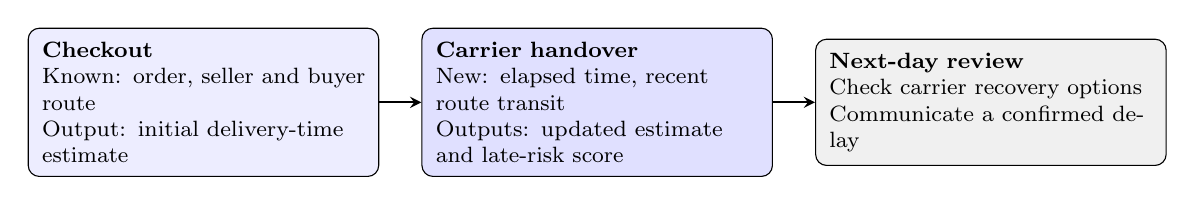
\begin{tikzpicture}[>=stealth,every node/.style={font=\footnotesize}]
\node[draw,rounded corners,fill=blue!7,align=left,text width=4.1cm,inner sep=5pt] (checkout) at (0,0) {\textbf{Checkout}\par Known: order, seller and buyer route\par Output: initial delivery-time estimate};
\node[draw,rounded corners,fill=blue!12,align=left,text width=4.1cm,inner sep=5pt] (handover) at (5.0,0) {\textbf{Carrier handover}\par New: elapsed time, recent route transit\par Outputs: updated estimate and late-risk score};
\node[draw,rounded corners,fill=gray!12,align=left,text width=4.1cm,inner sep=5pt] (action) at (10.0,0) {\textbf{Next-day review}\par Check carrier recovery options\par Communicate a confirmed delay};
\draw[->,thick] (checkout.east) -- (handover.west);
\draw[->,thick] (handover.east) -- (action.west);
\end{tikzpicture}
\caption{Prediction points and proposed action. Olist's original customer date anchors the late-risk label; delivery outcomes enter later model fits only after they are recorded.}
\label{fig:workflow}
\end{figure}

\section*{Model 1: Two-stage Delivery-time Estimate (Regression)}
\textbf{Method.} Both stages predict the same target, \texttt{delivery\_days}, on the same orders. Subtracting the purchase-to-handover time that has already elapsed from the handover prediction gives an estimate of remaining carrier days. The \textbf{checkout} stage uses the order, route and seller features known at purchase (20 inputs). The \textbf{handover} stage adds three inputs known once the carrier has the parcel: \texttt{handover\_days} (elapsed time), \texttt{approval\_days} (used only when approval was recorded by handover), and \texttt{route\_transit\_90d\_at\_handover} (the route's mean carrier-to-customer days over the previous 90 days, built only from deliveries already recorded, shrunk toward the all-route mean). Table~\ref{tab:ladder} holds ridge (\(\alpha=100\)) fixed while adding information; most of the improvement comes from observing elapsed time, while recent route history adds a smaller gain.

\begin{table}[ht]
\centering\small
\caption{Information ladder: Ridge regression (\(\alpha=100\)) throughout, same orders at every rung, mean over five validation windows.}
\label{tab:ladder}
\begin{tabular}{@{}lrrr@{}}
\toprule
Rung & MAE (days) & \(R^2\) & Lowest-window \(R^2\) \\
\midrule
Checkout (20 frozen inputs) & \LadderCheckoutMAE{} & \LadderCheckoutRSq{} & \LadderCheckoutMinRSq{} \\
+ recent route transit history & \LadderTransitMAE{} & \LadderTransitRSq{} & \LadderTransitMinRSq{} \\
+ elapsed days to handover and approval & \LadderElapsedMAE{} & \LadderElapsedRSq{} & \LadderElapsedMinRSq{} \\
Handover (history as of handover) & \LadderHandoverMAE{} & \LadderHandoverRSq{} & \LadderHandoverMinRSq{} \\
\bottomrule
\end{tabular}
\end{table}

\textbf{Candidates and selection.} MAE is our selection measure because it expresses the average absolute miss in days; RMSE highlights larger errors and $R^2$ compares explained variation. Within each family we climb in complexity only as far as the data rewards it: a training-mean floor, then plain linear regression and a single tree, then ridge penalties, tree pruning, random forest and gradient boosting. The latter two follow our Phase 1 review’s suggestion that non-linear effects might matter, but, as a rule, extra complexity is kept only if it earns its place on validation. At checkout, plain linear cuts MAE from the mean floor's \CheckoutMeanMAE{} to 5.86 days; ridge reaches \CheckoutSelMAE{}. A plain tree scores 7.79 days and improves to \CheckoutBestMAE{} with a forest. At handover, ridge improves on plain linear (5.15 to \HandoverSelMAE{} days), while the forest improves on the plain tree (6.84 to 5.35 days) but remains behind ridge. A transparent rule, elapsed days plus the route's recent carrier time, scores \HandoverRuleMAE{} days, so most of the handover gain comes from observing elapsed time and the model adds a further 0.2 days.

Across families, we adapt the one-standard-error simplicity rule~\cite{james2013}: choose the lowest mean validation MAE unless a simpler model's paired gap is within one standard error across the five windows. The checkout forest's advantage over ridge is only \CheckoutSelGap{} days (paired SE \CheckoutSelGapSE{}), so ridge $\alpha=100$ is selected there; at handover that ridge is itself the lowest-MAE candidate. An equal-weight ridge/boosting vote scores 5.11 days at handover, adding no improvement. The five windows make the SE approximate, but the selection itself does not depend on the later test period. Full comparisons appear in Appendix Table~\ref{tab:app-regression}.

\begin{figure}[ht]
\centering
% BEGIN GENERATED fig_ladder -- refreshed by phase2_final_evidence.py
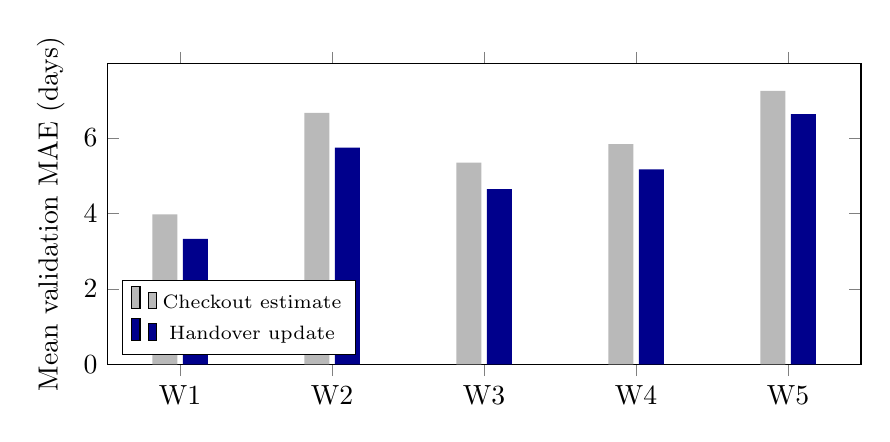
\begin{tikzpicture}
\begin{axis}[width=0.92\linewidth,height=5.4cm,ybar,bar width=9pt,ymin=0,ylabel={Mean validation MAE (days)},
 symbolic x coords={W1,W2,W3,W4,W5},xtick=data,enlarge x limits=0.12,legend style={at={(0.02,0.03)},anchor=south west,font=\scriptsize}]
\addplot[fill=gray!55,draw=none] coordinates {(W1,3.97) (W2,6.66) (W3,5.34) (W4,5.83) (W5,7.24)};
\addplot[fill=blue!55!black,draw=none] coordinates {(W1,3.32) (W2,5.74) (W3,4.64) (W4,5.16) (W5,6.63)};
\legend{Checkout estimate,Handover update}
\end{axis}
\end{tikzpicture}
% END GENERATED fig_ladder
\caption{Mean validation MAE by window, checkout estimate against the handover update (selected models). The handover update beats the checkout estimate in every window, including the higher-lateness windows.}
\label{fig:ladder}
\end{figure}

\textbf{Later-period results.} The handover update lowers the later-period MAE by about a day: \HandoverTestMAE{} days against \CheckoutTestMAE{} at checkout (RMSE \HandoverTestRMSE{} against \CheckoutTestRMSE{}; $R^2$ \HandoverTestRSq{} against \CheckoutTestRSq{}). Deliveries were faster in this period, so both models over-predicted, with mean signed errors of \HandoverTestBias{} and \CheckoutTestBias{} days (Appendix Figure~\ref{fig:test-bias}). The same shift explains the negative checkout $R^2$, which compares the model with the later period's own, lower mean. We therefore present the estimate as review context, not as a new customer date. A random split of the same orders would give the handover ridge an $R^2$ of \HandoverRandTestRSq{}, against \HandoverSelRSq{} across the chronological windows; the gap reflects shifting conditions rather than a different model, so random-split scores stay secondary (Appendix~\ref{app:diag}).

\textbf{What drives the estimate.} Among scaled numeric inputs, the largest mean absolute ridge coefficients at checkout belong to promised days (\CheckoutImpAVal{}), distance (\CheckoutImpBVal{}) and the route's typical delivery time (\CheckoutImpCVal{}). At handover, elapsed time leads (\HandoverImpAVal{}), matching the information ladder: knowing how long the order has already taken is the main reason to update its estimate. Correlated inputs mean these coefficients describe the fitted model, not causal effects.

\section*{Model 2: The Late Warning (Classification)}
\textbf{Candidates and selection.} Each family starts from its simplest version: plain logistic regression (validation PR-AUC \ClsPlainPR{}) and a single decision tree (0.137). We then tune regularisation, class weights, tree depth, random forests and gradient boosting. Logistic regression with strong regularisation ($C=0.01$) scores best, at \ValSelPR{}. Class weighting lowers it to 0.372, so we keep the natural share of late orders. The best random forest also reaches 0.372; it trails logistic regression by 0.011, more than the paired standard error of 0.004, so logistic regression wins outright (Table~\ref{tab:family-summary}). Walk-forward selection confirms the choice: choosing on earlier windows only picks the same model before each of the last three windows.

% BEGIN GENERATED fig_family_summary -- refreshed by phase2_final_evidence.py
\begin{table}[ht]
\centering\small
\caption{Classifiers by family, mean over five validation windows: the simplest version of each family and its best tuned version, against the remaining-slack rule. Every configuration is in Appendix Table~\ref{tab:app-classifier}.}
\label{tab:family-summary}
\begin{tabular}{@{}llrrr@{}}
\toprule
Family & Configuration & PR-AUC & ROC-AUC & Recall at top 10\% \\
\midrule
Linear & logistic\_unregularized (simplest) & 0.354 & 0.736 & 34\% \\
Linear & logistic\_c0.01 (best tuned) & 0.382 & 0.774 & 36\% \\
Tree & tree\_plain (simplest) & 0.137 & 0.559 & 21\% \\
Tree & tree\_d8\_l100 (best tuned) & 0.308 & 0.684 & 32\% \\
Forest & forest\_l50\_sqrt (best tuned) & 0.372 & 0.750 & 34\% \\
Boosting & boost\_lr0.03\_n200\_l20 (best tuned) & 0.356 & 0.743 & 33\% \\
Rule & remaining slack (benchmark) & 0.328 & 0.697 & 30\% \\
\bottomrule
\end{tabular}
\end{table}
% END GENERATED fig_family_summary

\textbf{Benchmark: the remaining-slack rule.} Without a model, staff could rank parcels by remaining slack: promised days minus days elapsed minus the route's recent carrier time. The model must beat this rule to be worth deploying. On validation it does, with PR-AUC \ValSelPR{} against \RuleValPR{}. It wins all five windows, and the 95\% bootstrap interval for the gap (\RuleGapLow{} to \RuleGapHigh{}) excludes zero.

Two engineered inputs make this possible: whether the promised date had already passed at handover, and the slack shortfall, $\max(0,-\text{slack})$ days. Lateness becomes near-certain once slack runs out (\PastPromiseLateRate{}\% of orders already past their date were late in validation), but logistic regression is linear in slack and cannot express that jump on its own. Without these inputs the same model scores \ShapeValWithout{} on validation and \ShapeTestWithout{} in the later test period, instead of \ShapeValWith{} and \ShapeTestWith{}. We keep them because they improve every validation window.

\textbf{Imbalance and metrics.} Late orders are rare: \ClsTestLate{}\% in the later test period and 4--21\% across validation windows, so accuracy would mislead. We select by PR-AUC and report each period's late rate as its random-ranking baseline~\cite{saito2015}. We also report ROC-AUC, and precision, recall and F1 for a review list of fixed size. Per-window results, ROC and precision--recall curves, and confusion counts with MCC are in Appendix~\ref{app:diag}.

\textbf{Value across periods.} Table~\ref{tab:period-value} compares the model and the rule at the same workload in every period. The model finds more late orders in all five validation windows: \CalmGainMin{}--\CalmGainMax{}\% more in the calm windows and \BusyGainMin{}--\BusyGainMax{}\% more in the busy ones. Across the four periods evaluated after the model was chosen (W3--W5 and the later test period), it finds \OosModelCaught{} late orders against the rule's \OosRuleCaught{}, \OosGainPct{}\% more.

% BEGIN GENERATED fig_period_value -- refreshed by phase2_final_evidence.py
\begin{table}[ht]
\centering\small
\caption{Model against the remaining-slack rule at the same workload: the top \ActShare{}\% of each window, or of each purchase month in the later test period (Later). W3--W5 and the later test period were evaluated after the model was chosen on earlier windows. A random list would catch \ActShare{}\% of late orders.}
\label{tab:period-value}
\begin{tabular}{@{}lrrrrrrr@{}}
\toprule
& & Late already & \multicolumn{2}{c}{PR-AUC} & \multicolumn{3}{c}{Late orders caught} \\
\cmidrule(lr){4-5}\cmidrule(l){6-8}
Period & Late rate & past date & Model & Rule & Model & Rule & Random \\
\midrule
W1 & 4.1\% & 12\% & 0.374 & 0.354 & 175 & 153 & 40 \\
W2 & 13.8\% & 6\% & 0.416 & 0.343 & 401 & 313 & 137 \\
W3 & 4.8\% & 7\% & 0.281 & 0.256 & 146 & 117 & 47 \\
W4 & 9.9\% & 3\% & 0.356 & 0.301 & 318 & 257 & 98 \\
W5 & 20.7\% & 1\% & 0.483 & 0.386 & 533 & 443 & 205 \\
Later & 3.5\% & 29\% & 0.477 & 0.519 & 387 & 424 & 87 \\
\bottomrule
\end{tabular}
\end{table}
% END GENERATED fig_period_value

\textbf{The later test period and data drift.} In the later test period, the model's top 10\% still holds \GainTenModel{}\% of late orders, more than five times a random list (Figure~\ref{fig:gains}). The rule, however, finds slightly more late orders (\LaterRuleCaught{} against \LaterModelCaught{}). Both rank every parcel already past its promise at the top, so the gap lies in parcels that still had time, and almost all of it arose in August. That month the data drifted. Olist's monthly average promise had stayed between \PromSpanMin{} and \PromSpanMax{} days from March 2017 to May 2018; in August it fell to \PromAug{}, and \ShortShareAug{}\% of orders had promises under \ShortCut{} days, the shortest tenth of training promises. On these short-promise orders the model had never clearly beaten the rule: it was ahead in \ShortValModelWins{} of five validation windows, and behind in the later test period (PR-AUC \ShortTestPRModel{} against \ShortTestPRRule{}).

We tested three responses to the drift, each compared on validation first: monthly retraining, removing the raw promise inputs, and a rule-first model allowed only to adjust the slack score (Appendix~\ref{app:remedies}). None overtook the rule in August. The underlying limit is feedback lag: the model learns only from delivered orders, and on 1 August only about one in ten orders with known outcomes had a short promise. The rule needs no history, which makes it the right fallback during drift.

\begin{figure}[ht]
\centering
% BEGIN GENERATED fig_gains -- refreshed by phase2_final_evidence.py
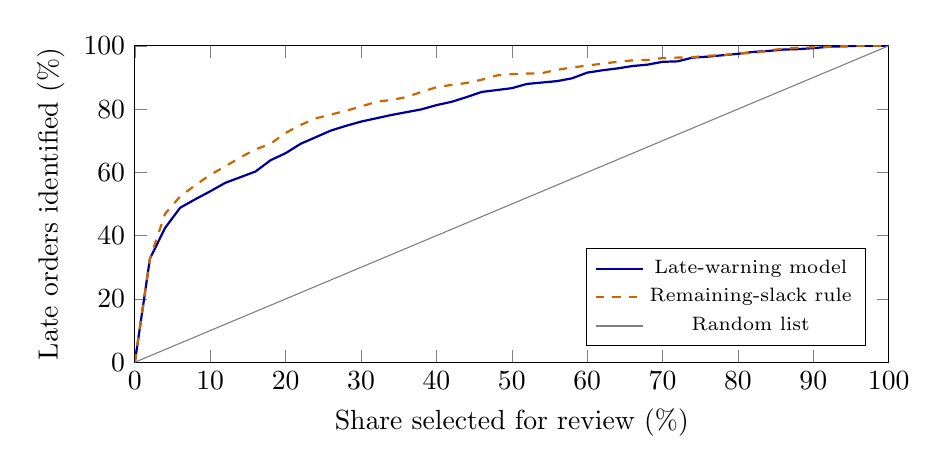
\begin{tikzpicture}
\begin{axis}[width=0.92\linewidth,height=5.6cm,xlabel={Share selected for review (\%)},ylabel={Late orders identified (\%)},
 xmin=0,xmax=100,ymin=0,ymax=100,legend style={at={(0.97,0.05)},anchor=south east,font=\scriptsize}]
\addplot[thick,blue!60!black,no marks] coordinates {(0.0,0.0000) (2.0,32.7381) (4.0,42.4107) (6.0,48.8095) (8.0,51.4881) (10.0,54.0179) (12.0,56.6964) (14.000000000000002,58.4821) (16.0,60.2679) (18.0,63.8393) (20.0,66.0714) (22.0,69.0476) (24.0,71.1310) (26.0,73.2143) (28.000000000000004,74.7024) (30.0,76.0417) (32.0,77.0833) (34.0,78.1250) (36.0,79.0179) (38.0,79.9107) (40.0,81.2500) (42.0,82.2917) (44.0,83.7798) (46.0,85.4167) (48.0,86.0119) (50.0,86.6071) (52.0,87.9464) (54.0,88.3929) (56.00000000000001,88.8393) (57.99999999999999,89.7321) (60.0,91.5179) (62.0,92.2619) (64.0,92.8571) (66.0,93.6012) (68.0,94.0476) (70.0,94.9405) (72.0,95.0893) (74.0,96.2798) (76.0,96.5774) (78.0,97.0238) (80.0,97.4702) (82.0,98.0655) (84.0,98.3631) (86.0,98.8095) (88.0,98.9583) (90.0,99.2560) (92.0,99.7024) (94.0,99.8512) (96.0,100.0000) (98.0,100.0000) (100.0,100.0000)};
\addlegendentry{Late-warning model}
\addplot[thick,orange!80!black,dashed,no marks] coordinates {(0.0,0.0000) (2.0,32.7381) (4.0,46.8750) (6.0,52.3810) (8.0,55.9524) (10.0,59.2262) (12.0,61.9048) (14.000000000000002,64.7321) (16.0,67.2619) (18.0,69.0476) (20.0,72.4702) (22.0,75.0000) (24.0,77.0833) (26.0,78.2738) (28.000000000000004,79.4643) (30.0,80.8036) (32.0,82.2917) (34.0,82.8869) (36.0,83.7798) (38.0,85.4167) (40.0,86.9048) (42.0,87.6488) (44.0,88.2440) (46.0,89.2857) (48.0,90.6250) (50.0,91.0714) (52.0,91.2202) (54.0,91.3690) (56.00000000000001,92.4107) (57.99999999999999,93.1548) (60.0,93.7500) (62.0,94.3452) (64.0,94.9405) (66.0,95.3869) (68.0,95.5357) (70.0,96.1310) (72.0,96.2798) (74.0,96.4286) (76.0,96.8750) (78.0,97.0238) (80.0,97.6190) (82.0,97.6190) (84.0,98.5119) (86.0,99.1071) (88.0,99.4048) (90.0,99.5536) (92.0,99.7024) (94.0,99.8512) (96.0,100.0000) (98.0,100.0000) (100.0,100.0000)};
\addlegendentry{Remaining-slack rule}
\addplot[thin,gray,no marks] coordinates {(0.0,0.0000) (2.0,2.0000) (4.0,4.0000) (6.0,6.0000) (8.0,8.0000) (10.0,10.0000) (12.0,12.0000) (14.000000000000002,14.0000) (16.0,16.0000) (18.0,18.0000) (20.0,20.0000) (22.0,22.0000) (24.0,24.0000) (26.0,26.0000) (28.000000000000004,28.0000) (30.0,30.0000) (32.0,32.0000) (34.0,34.0000) (36.0,36.0000) (38.0,38.0000) (40.0,40.0000) (42.0,42.0000) (44.0,44.0000) (46.0,46.0000) (48.0,48.0000) (50.0,50.0000) (52.0,52.0000) (54.0,54.0000) (56.00000000000001,56.0000) (57.99999999999999,58.0000) (60.0,60.0000) (62.0,62.0000) (64.0,64.0000) (66.0,66.0000) (68.0,68.0000) (70.0,70.0000) (72.0,72.0000) (74.0,74.0000) (76.0,76.0000) (78.0,78.0000) (80.0,80.0000) (82.0,82.0000) (84.0,84.0000) (86.0,86.0000) (88.0,88.0000) (90.0,90.0000) (92.0,92.0000) (94.0,94.0000) (96.0,96.0000) (98.0,98.0000) (100.0,100.0000)};
\addlegendentry{Random list}
\end{axis}
\end{tikzpicture}
% END GENERATED fig_gains
\caption{Later test period: share of late orders caught against share of orders reviewed, ranking within each purchase month.}
\label{fig:gains}
\end{figure}

\textbf{Size and value of the review list.} With no cost data, we assumed that a caught late order is worth \BenefitRatio{} reviews. Under that assumption the best list on validation covers \ActShare{}\% of handovers, but the choice is sensitive: a ratio of two picks 1\%, and a ratio of ten picks 30\%. We therefore also report break-even values. At \ActShare{}\%, about 1 in \BreakEvenVal{} listed orders was late in validation and 1 in \BreakEvenTest{} in the later test period (Table~\ref{tab:classifier-test}). The list pays off when rescuing a late order is worth more than about three reviews in busy periods, or six to seven in calm ones. List size is therefore a business decision, and a list sized for a busy season can overspend in a quieter one.

\begin{table}[ht]
\centering\small
\caption{Later test period: ranking quality and the top-\ActShare{}\% review list, drawn within each purchase month (which uses scores from later in the month; the daily replay applies it day by day). PR-AUC and ROC-AUC use all orders; precision, recall and F1 use the review list.}
\label{tab:classifier-test}
\begin{tabular}{@{}lccccc@{}}
\toprule
& PR-AUC & ROC-AUC & Precision & Recall & F1 \\
\midrule
Late-warning model & \ClsTestPR{} & \ClsTestROC{} & \ClsTestPrec{}\% & \ClsTestRec{}\% & \ClsTestFone{} \\
Remaining-slack rule & \RuleTestPR{} & \RuleTestROC{} & \RuleTestPrec{}\% & \RuleTestRec{}\% & \RuleTestFone{} \\
Random list & \ClsTestLate{}\% & 0.50 & \ClsTestLate{}\% & \ActShare{}\% & --- \\
\bottomrule
\end{tabular}
\end{table}

\textbf{Daily replay.} Applied day by day over the later test period, the \ActShare{}\% list flags a median of \FullDailyMedianFlagged{} parcels a day and finds \FullDailyCaught{} of \FullDailyLate{} late orders (\FullDailyRecall{}\% recall). By 9am the next day, \FullDailyBeforePromise{} of these were still before their promised date, leaving time to act (Appendix Table~\ref{tab:daily-replay}).

\textbf{What drives the score.} Shuffling one input at a time on validation~\cite{breiman2001}, the largest PR-AUC drops come from slack shortfall (\ImpADrop{}), days elapsed (\ImpBDrop{}) and remaining slack (\ImpCDrop{}); every other input contributes under 0.02. The model mainly reads how far an order has fallen behind its promise, which only becomes visible at handover.

\section*{Proposed Operations Workflow}
\begin{enumerate}\setlength{\itemsep}{0pt}
\item \textbf{Each day at handover}, score every new parcel for late risk against its promised date and estimate its remaining delivery time. Rank the day's parcels for review the next morning. If the model is unavailable, rank by remaining slack instead.
\item \textbf{Each morning}, staff check the top of the list, up to a capacity operations chooses, with the remaining-time estimate to hand. Orders already past their date get an immediate update to the customer. For the rest, staff ask the carrier whether a faster service or another recovery option exists, and at what cost.
\item \textbf{Each month}, track whether the delivery estimate runs consistently long or short, the late rate, the length of Olist's promises, and how many flagged orders turn out late. A sustained change, or a change in how Olist sets promises, is the signal to retrain the models or resize the list. If the data drifts sharply, as promise lengths did in August 2018, switch to the rule until the model has been retrained on enough of the new orders. The pilot should test this switch.
\end{enumerate}

\section*{Limitations and Pilot Requirements}
\begin{itemize}\setlength{\itemsep}{0pt}
\item \textbf{Conditions change.} About \NormalLate{}\% of orders are late in ordinary months, but \BlackFridayLate{}\% were late around Black Friday and \FebMarLate{}\% in February--March 2018 (Appendix Figure~\ref{fig:monthly}). Olist's promises had stayed between \PromSpanMin{} and \PromSpanMax{} days a month from March 2017 to May 2018, then fell to \PromJul{} days in July and \PromAug{} in August 2018, shorter than in any earlier month. Models trained on one period carry its habits into the next: both regressions predicted deliveries about three days too long in the faster later period. That is why the workflow reviews performance monthly instead of fixing the models and the list size once.
\item \textbf{Cohort.} Results describe orders that were eventually delivered with a recorded carrier handover; cancelled and still-open orders have no outcome and are not covered.
\item \textbf{Intervention outcomes.} Olist's data do not record carrier recovery options, their costs, or effects on delivery and reviews. A pilot with a control group would test whether acting on the scores improves outcomes enough to justify its cost.
\end{itemize}

\section*{Declaration on the Use of AI}
Claude (Anthropic) and OpenAI Codex assisted with analysis code, figures and report drafting. The student authors are responsible for checking the calculations, citations and final submission.

\begin{thebibliography}{99}\small\setlength{\itemsep}{0pt}
\bibitem{bergmeir2012} C.~Bergmeir and J.~M.~Ben\'itez. On the use of cross-validation for time series predictor evaluation. \emph{Information Sciences}, 2012. doi:10.1016/j.ins.2011.12.028.
\bibitem{breiman2001} L.~Breiman. Random forests. \emph{Machine Learning}, 45(1):5--32, 2001.
\bibitem{dearaujo2021} A.~C.~de Araujo and A.~Etemad. End-to-end prediction of parcel delivery time with deep learning for smart-city applications. \emph{IEEE Internet of Things Journal}, 8(23):17043--17056, 2021. doi:10.1109/JIOT.2021.3077007.
\bibitem{gibellini2024} F.~Gibellini, B.~van Gool, M.~Firat and S.~Bromuri. Estimating the time of arrival of a shipment with machine learning. \emph{ECAI 2024}, pp.~4681--4688. doi:10.3233/FAIA241064.
\bibitem{james2013} G.~James, D.~Witten, T.~Hastie and R.~Tibshirani. \emph{An Introduction to Statistical Learning}, Sec.~6.1.3, p.~214. Springer, 2013.
\bibitem{saito2015} T.~Saito and M.~Rehmsmeier. The precision-recall plot is more informative than the ROC plot when evaluating binary classifiers on imbalanced datasets. \emph{PLOS ONE}, 10(3):e0118432, 2015.
\bibitem{salari2022} N.~Salari, S.~Liu and Z.-J.~M.~Shen. Real-time delivery time forecasting and promising in online retailing: when will your package arrive? \emph{Manufacturing \& Service Operations Management}, 24(3):1421--1436, 2022.
\end{thebibliography}

\clearpage
\appendix
\section{Prepared-table validation}
\label{app:gx}
Before the delivery-sequence exclusions, a Great Expectations (GX Core 1.24.0) suite checked the 96,470-row prepared order table. Its saved run passed all 35 expectations: eight identity, target and split checks; one exact-column-set check; 16 value-range checks; five category checks; and five missingness checks. Separate timestamp checks confirmed that fitting outcomes were recorded by the 26 May 2018 cutoff. The model comparison uses 96,272 orders after excluding 198 rows without a valid purchase--carrier--delivery sequence.

\begin{table}[ht]
\centering\small
\caption{Prepared-table validation and later-period feature checks. The 35 contract checks apply before the final sequence filter; monthly feature checks are separate diagnostics.}
\label{tab:gx}
\begin{tabular}{@{}lr@{}}
\toprule
Check & Saved result \\
\midrule
Identity, targets and split & 8/8 passed \\
Exact column set & 1/1 passed \\
Value ranges and categories & 21/21 passed \\
Documented missingness & 5/5 passed \\
Later monthly feature means outside training range & 5 of 21 \\
\bottomrule
\end{tabular}
\end{table}

The five out-of-range means are June freight, July promised days and freight, and August promised days and historical seller handover time. They document a change in the observed feature mix, not its cause. An exact column set can catch an unapproved predictor, but cannot establish when a historical value became known; the point-in-time feature construction is checked separately.

\section{Delivery context and diagnostics}
\label{app:diag}
\begin{table}[H]
\centering\small
\caption{Retrospective purchase-month test ranking at the validation-selected \ActShare{}\% share. Counts describe model selection for review, not carrier interventions.}
\label{tab:classifier-monthly}
\begin{tabular}{@{}lrrrr@{}}
\toprule
Month & Orders & Late orders & Flagged & Late caught \\
\midrule
May (from the 26th) & \TestMayOrders{} & \TestMayLateCount{} & \TestMayActed{} & \TestMayCaught{} \\
June & \TestJunOrders{} & \TestJunLateCount{} & \TestJunActed{} & \TestJunCaught{} \\
July & \TestJulOrders{} & \TestJulLateCount{} & \TestJulActed{} & \TestJulCaught{} \\
August & \TestAugOrders{} & \TestAugLateCount{} & \TestAugActed{} & \TestAugCaught{} \\
\bottomrule
\end{tabular}
\end{table}
% BEGIN GENERATED fig_classifier_windows -- refreshed by phase2_final_evidence.py
\begin{table}[H]
\centering\small
\caption{The selected classifier in each validation window. The late rate of each window is the PR-AUC of a random list.}
\label{tab:classifier-windows}
\begin{tabular}{@{}lrrrrr@{}}
\toprule
Window & Orders & Late rate & PR-AUC & ROC-AUC & Top-10\% precision \\
\midrule
W1 & 7,600 & 4.1\% & 0.374 & 0.811 & 20.8\% \\
W2 & 7,601 & 13.8\% & 0.416 & 0.768 & 43.8\% \\
W3 & 7,601 & 4.8\% & 0.281 & 0.750 & 16.6\% \\
W4 & 7,601 & 9.9\% & 0.356 & 0.780 & 34.6\% \\
W5 & 7,600 & 20.7\% & 0.483 & 0.759 & 57.2\% \\
\bottomrule
\end{tabular}
\end{table}
% END GENERATED fig_classifier_windows
% BEGIN GENERATED fig_split_summary -- refreshed by phase2_final_evidence.py
\begin{table}[H]
\centering\small
\caption{Chosen models on training data, validation (mean of five windows) and the later test period. The periods differ in late rate.}
\label{tab:split-summary}
\begin{tabular}{@{}lrrr@{}}
\toprule
Metric & Training & Validation & Final test \\
\midrule
Checkout MAE (days) & 5.23 & 5.81 & 5.00 \\
Handover MAE (days) & 4.57 & 5.10 & 3.97 \\
Late warning PR-AUC & 0.344 & 0.382 & 0.477 \\
Late prevalence & 7.1\% & 10.7\% & 3.5\% \\
\bottomrule
\end{tabular}
\end{table}
% END GENERATED fig_split_summary
% BEGIN GENERATED fig_complete_daily_replay -- refreshed by phase2_final_evidence.py
\begin{table}[H]
\centering\small
\caption{Day-by-day replay of the chosen model, flagging the top \ActShare{}\% of handovers each day. Each row covers every valid handover in its calendar span. Counts show which orders would be flagged, not the effect of acting on them.}
\label{tab:daily-replay}
\begin{tabular}{@{}lrrrrrr@{}}
\toprule
Period & Active days & Orders & Late rate & Median flagged/day & Precision & Recall \\
\midrule
W1 & 45 & 7,262 & 3.6\% & 25 & 14.3\% & 52.5\% \\
W2 & 24 & 7,450 & 12.9\% & 47 & 36.3\% & 37.0\% \\
W3 & 33 & 7,685 & 5.7\% & 34 & 19.2\% & 44.6\% \\
W4 & 28 & 7,591 & 9.1\% & 42 & 26.3\% & 38.1\% \\
W5 & 29 & 7,357 & 21.9\% & 38 & 56.2\% & 34.1\% \\
Later test & 81 & 19,534 & 3.6\% & 36 & 16.0\% & 58.7\% \\
\bottomrule
\end{tabular}
\end{table}
% END GENERATED fig_complete_daily_replay
\textbf{Same-period diagnostic.} A secondary random five-fold validation and 20\% test yield checkout \(R^2\) \CheckoutRandValRSq{} / \CheckoutRandTestRSq{} (test MAE \CheckoutRandTestMAE{}) and handover \(R^2\) \HandoverRandValRSq{} / \HandoverRandTestRSq{} (test MAE \HandoverRandTestMAE{}). These interpolate within one period and were not used for model selection; their stronger scores illustrate the cost of temporal shift.
\begin{figure}[H]
\centering
% BEGIN GENERATED fig_monthly -- refreshed by phase2_final_evidence.py
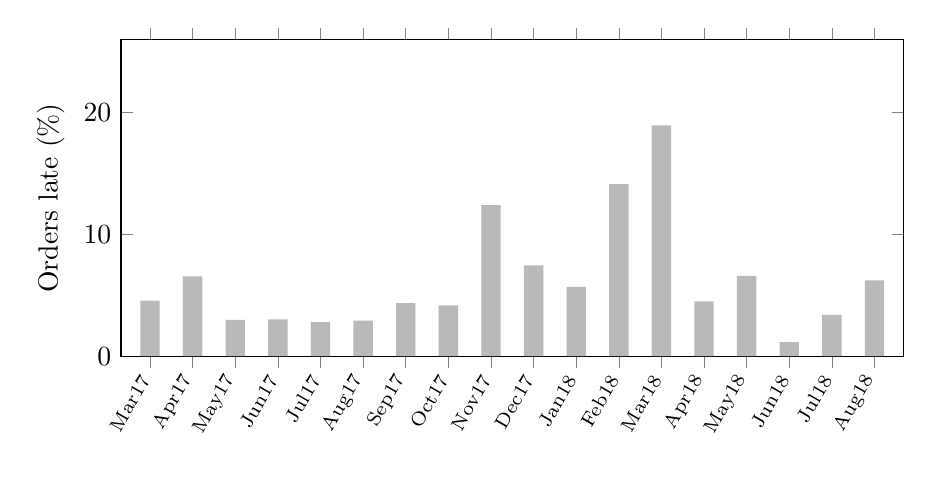
\begin{tikzpicture}
\begin{axis}[width=0.95\linewidth,height=5.6cm,ybar,bar width=7pt,ymin=0,ymax=26,ylabel={Orders late (\%)},
 symbolic x coords={Mar17,Apr17,May17,Jun17,Jul17,Aug17,Sep17,Oct17,Nov17,Dec17,Jan18,Feb18,Mar18,Apr18,May18,Jun18,Jul18,Aug18},xtick=data,x tick label style={rotate=60,anchor=east,font=\scriptsize},
 enlarge x limits=0.04]
\addplot[fill=gray!55,draw=none] coordinates {(Mar17,4.558) (Apr17,6.557) (May17,2.991) (Jun17,3.031) (Jul17,2.799) (Aug17,2.912) (Sep17,4.362) (Oct17,4.176) (Nov17,12.404) (Dec17,7.455) (Jan18,5.701) (Feb18,14.127) (Mar18,18.966) (Apr18,4.506) (May18,6.593) (Jun18,1.157) (Jul18,3.383) (Aug18,6.232)};
\end{axis}
\end{tikzpicture}
% END GENERATED fig_monthly
\caption{Share of orders late by purchase month. Black Friday (November 2017) and February--March 2018 stand out as the clearest swings in delivery conditions; the June--August 2018 test months at right were calmer at \ClsTestLate{}\% late.}
\label{fig:monthly}
\end{figure}


\begin{figure}[H]
\centering
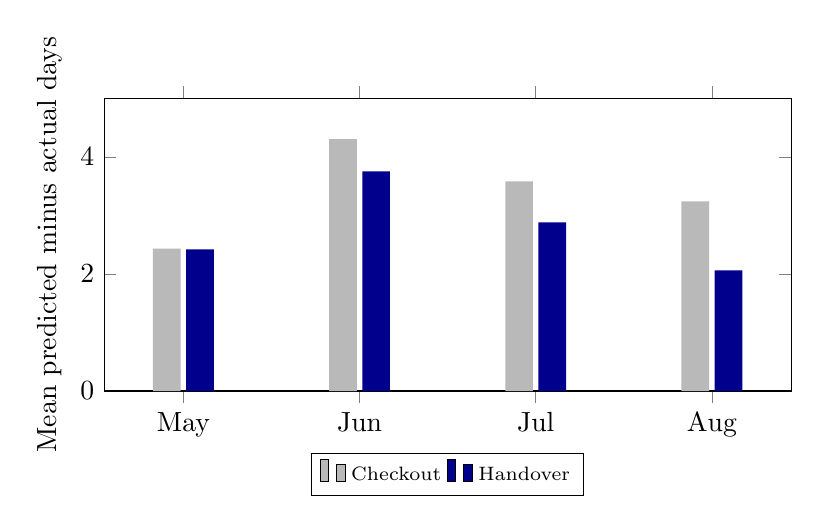
\begin{tikzpicture}
\begin{axis}[width=0.85\linewidth,height=5.3cm,ybar,bar width=10pt,ymin=0,ymax=5,
 symbolic x coords={May,Jun,Jul,Aug},xtick=data,enlarge x limits=0.15,
 ylabel={Mean predicted minus actual days},
 legend style={at={(0.5,-0.21)},anchor=north,legend columns=2,font=\scriptsize}]
\addplot[fill=gray!55,draw=none] coordinates {(May,2.43) (Jun,4.30) (Jul,3.58) (Aug,3.24)};
\addplot[fill=blue!55!black,draw=none] coordinates {(May,2.42) (Jun,3.75) (Jul,2.88) (Aug,2.06)};
\legend{Checkout,Handover}
\end{axis}
\end{tikzpicture}
\caption{Signed forecast error by purchase month in the later test period (May starts on the 26th). Positive values mean predicted delivery is later than actual delivery. This diagnoses the shift to faster deliveries; it was not used for model selection.}
\label{fig:test-bias}
\end{figure}

% BEGIN GENERATED fig_roc_pr -- refreshed by phase2_final_evidence.py
\begin{figure}[H]
\centering
\begin{minipage}{0.49\linewidth}\centering
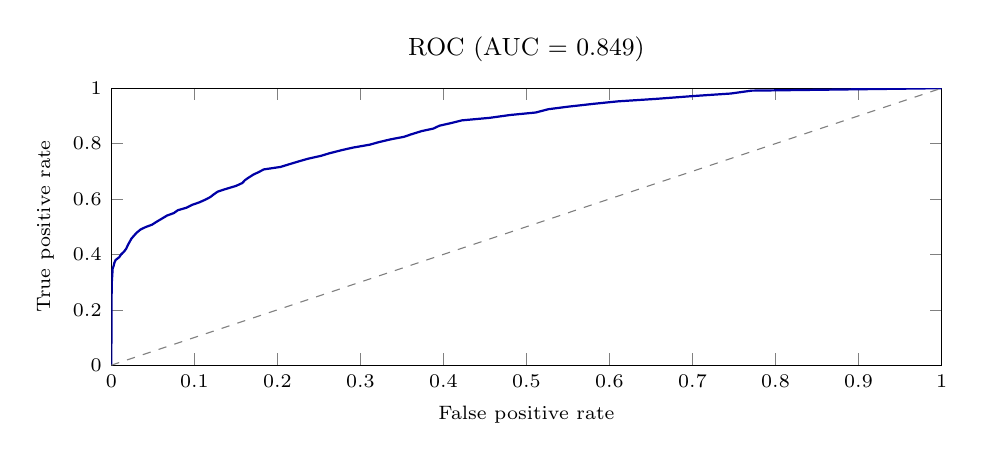
\begin{tikzpicture}
\begin{axis}[width=\linewidth,height=5.1cm,xmin=0,xmax=1,ymin=0,ymax=1,title style={font=\small},tick label style={font=\scriptsize},label style={font=\scriptsize},xlabel={False positive rate},ylabel={True positive rate},title={ROC (AUC = 0.849)}]
\addplot[thick,blue!65!black,no marks] coordinates {(0.0000,0.0000) (0.0003,0.2440) (0.0007,0.3036) (0.0012,0.3274) (0.0016,0.3482) (0.0028,0.3586) (0.0036,0.3690) (0.0051,0.3795) (0.0095,0.3899) (0.0119,0.4003) (0.0155,0.4107) (0.0180,0.4211) (0.0198,0.4330) (0.0220,0.4449) (0.0242,0.4568) (0.0272,0.4673) (0.0303,0.4777) (0.0351,0.4896) (0.0412,0.4985) (0.0491,0.5074) (0.0546,0.5179) (0.0613,0.5298) (0.0671,0.5402) (0.0752,0.5491) (0.0802,0.5595) (0.0904,0.5685) (0.0974,0.5789) (0.1059,0.5878) (0.1137,0.5982) (0.1193,0.6071) (0.1231,0.6161) (0.1281,0.6265) (0.1371,0.6354) (0.1502,0.6473) (0.1578,0.6577) (0.1610,0.6682) (0.1654,0.6771) (0.1707,0.6875) (0.1770,0.6964) (0.1837,0.7068) (0.2039,0.7158) (0.2151,0.7262) (0.2267,0.7366) (0.2371,0.7455) (0.2528,0.7560) (0.2625,0.7649) (0.2781,0.7768) (0.2913,0.7857) (0.3113,0.7961) (0.3220,0.8051) (0.3367,0.8155) (0.3524,0.8244) (0.3611,0.8333) (0.3739,0.8452) (0.3879,0.8542) (0.3952,0.8646) (0.4084,0.8735) (0.4224,0.8839) (0.4555,0.8929) (0.4806,0.9033) (0.5112,0.9122) (0.5264,0.9241) (0.5494,0.9330) (0.5807,0.9435) (0.6099,0.9524) (0.6556,0.9613) (0.7013,0.9717) (0.7461,0.9807) (0.7710,0.9911) (1.0000,1.0000)};
\addplot[thin,gray,dashed,no marks] coordinates {(0,0) (1,1)};
\end{axis}
\end{tikzpicture}
\end{minipage}\hfill
\begin{minipage}{0.49\linewidth}\centering
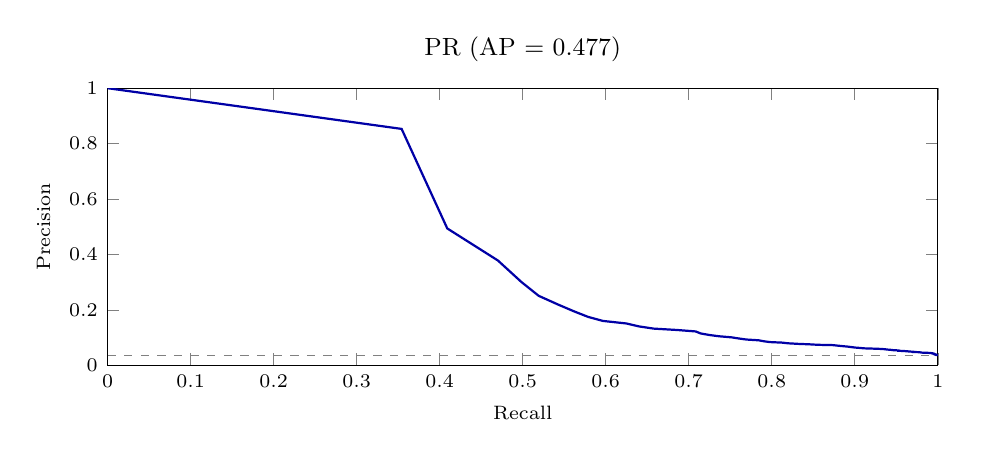
\begin{tikzpicture}
\begin{axis}[width=\linewidth,height=5.1cm,xmin=0,xmax=1,ymin=0,ymax=1,title style={font=\small},tick label style={font=\scriptsize},label style={font=\scriptsize},xlabel={Recall},ylabel={Precision},title={PR (AP = 0.477)}]
\addplot[thick,blue!65!black,no marks] coordinates {(0.0000,1.0000) (0.3542,0.8530) (0.4092,0.4937) (0.4702,0.3780) (0.4985,0.3004) (0.5193,0.2505) (0.5432,0.2183) (0.5625,0.1937) (0.5789,0.1744) (0.5967,0.1599) (0.6250,0.1507) (0.6399,0.1402) (0.6577,0.1322) (0.6860,0.1272) (0.7083,0.1220) (0.7143,0.1148) (0.7247,0.1092) (0.7366,0.1045) (0.7515,0.1007) (0.7604,0.0965) (0.7693,0.0928) (0.7842,0.0900) (0.7902,0.0866) (0.7976,0.0836) (0.8125,0.0816) (0.8199,0.0791) (0.8318,0.0771) (0.8452,0.0755) (0.8557,0.0737) (0.8735,0.0726) (0.8795,0.0707) (0.8854,0.0689) (0.8914,0.0672) (0.8958,0.0655) (0.9003,0.0638) (0.9062,0.0624) (0.9107,0.0610) (0.9211,0.0600) (0.9301,0.0590) (0.9360,0.0579) (0.9390,0.0566) (0.9435,0.0555) (0.9464,0.0543) (0.9524,0.0534) (0.9524,0.0522) (0.9583,0.0514) (0.9628,0.0505) (0.9658,0.0495) (0.9702,0.0487) (0.9702,0.0477) (0.9777,0.0471) (0.9792,0.0463) (0.9807,0.0455) (0.9866,0.0449) (0.9911,0.0443) (0.9926,0.0435) (0.9940,0.0428) (0.9940,0.0420) (0.9955,0.0414) (0.9955,0.0407) (0.9955,0.0400) (0.9970,0.0394) (0.9970,0.0388) (0.9970,0.0382) (0.9985,0.0376) (0.9985,0.0370) (1.0000,0.0365) (1.0000,0.0360) (1.0000,0.0355) (1.0000,0.0349)};
\addplot[thin,gray,dashed,no marks] coordinates {(0,0.0349) (1,0.0349)};
\end{axis}
\end{tikzpicture}
\end{minipage}
\caption{Final handover logistic classifier on 19,230 later-test-period orders (672 late). Curves are sampled points for display; AUC and average precision (AP) use all predictions. Dashed lines show random ranking. The top-\ActShare{}\% review list is drawn separately each month, so it is not a single point on these curves.}
\label{fig:roc-pr}
\end{figure}
% END GENERATED fig_roc_pr

% BEGIN GENERATED fig_confusion -- refreshed by phase2_final_evidence.py
\begin{table}[H]
\centering\small
\caption{Later test period confusion counts for the top-\ActShare{}\% monthly review list. Counts show who would be flagged, before any action is taken.}
\label{tab:app-confusion}
\begin{tabular}{@{}lrr@{}}
\toprule
& Actually late & Actually on time \\
\midrule
Selected for review & 387 & 2,115 \\
Not selected & 285 & 16,443 \\
\bottomrule
\end{tabular}
\end{table}
% END GENERATED fig_confusion

At this review share, MCC is \ClsTestMCC{} (zero indicates no association between selection and lateness).

\section{Remedies tested for the August gap}
\label{app:remedies}
These additional checks investigate the August gap. Each was compared on the validation windows before the later period, and none changed the selected model. They use a top-10\% review list, so their counts differ slightly from the main tables; the monthly-retraining check groups lists by handover month and the others by purchase month, so the rule's count differs between them. Code and outputs are in the repository's \texttt{experiments/monthly\_retraining/} and \texttt{experiments/promise\_dependence/} folders.

\begin{table}[H]
\centering\small
\caption{Late orders caught by each remedy against the current model and the remaining-slack rule. $^{*}$On validation, monthly retraining is compared with quarterly retraining; in the later period, with the single model trained in May. ``August short'' counts August orders with promises under \ShortCut{} days that were still before their date at handover (208 late, 336 reviews).}
\label{tab:remedies}
\begin{tabular}{@{}lrrr@{}}
\toprule
Remedy & Validation & Later period & August short \\
& remedy / current & remedy / current / rule & remedy / current / rule \\
\midrule
Monthly retraining$^{*}$ & 1,275 / 1,212 & 375 / 364 / 394 & 67 / 61 / 73 \\
Raw promise inputs removed & 1,321 / 1,315 & 363 / 363 / 398 & 61 / 61 / 73 \\
\quad and promise reconstruction blocked & 1,306 / 1,315 & 362 / 363 / 398 & 58 / 61 / 73 \\
Rule-first model with a bounded correction & 1,314 / 1,315 & 364 / 363 / 398 & 50 / 61 / 73 \\
\bottomrule
\end{tabular}
\end{table}

\section{Full configuration tables}
% BEGIN GENERATED fig_appendix_regression -- refreshed by phase2_final_evidence.py
\begin{table}[H]
\centering\small
\caption{Every regression candidate, mean over five validation windows.}
\label{tab:app-regression}
\begin{tabular}{@{}lllrrr@{}}
\toprule
Stage & Candidate & Family & MAE & RMSE & $R^2$ \\
\midrule
Checkout & mean\_baseline & mean & 7.215 & 10.671 & -0.078 \\
Checkout & linear\_baseline & linear & 5.860 & 9.464 & 0.155 \\
Checkout & ridge\_1 & ridge & 5.858 & 9.462 & 0.156 \\
Checkout & ridge\_10 & ridge & 5.848 & 9.451 & 0.158 \\
Checkout & ridge\_100 & ridge & 5.809 & 9.398 & 0.167 \\
Checkout & tree\_baseline & tree & 7.787 & 12.344 & -0.472 \\
Checkout & tree\_depth6 & tree & 5.933 & 9.505 & 0.144 \\
Checkout & forest\_leaf20 & forest & 5.783 & 9.340 & 0.176 \\
Checkout & boost\_baseline & boost & 5.830 & 9.452 & 0.155 \\
Checkout & boost\_slow & boost & 5.816 & 9.444 & 0.157 \\
Handover & mean\_baseline & mean & 7.215 & 10.671 & -0.078 \\
Handover & elapsed\_plus\_route\_baseline & rule & 5.304 & 8.396 & 0.337 \\
Handover & linear\_baseline & linear & 5.146 & 8.472 & 0.327 \\
Handover & ridge\_1 & ridge & 5.145 & 8.470 & 0.327 \\
Handover & ridge\_10 & ridge & 5.136 & 8.460 & 0.329 \\
Handover & ridge\_100 & ridge & 5.099 & 8.406 & 0.338 \\
Handover & tree\_baseline & tree & 6.840 & 11.625 & -0.330 \\
Handover & tree\_depth6 & tree & 5.313 & 8.633 & 0.299 \\
Handover & forest\_leaf20 & forest & 5.346 & 8.808 & 0.270 \\
Handover & boost\_baseline & boost & 5.214 & 8.651 & 0.297 \\
Handover & boost\_slow & boost & 5.215 & 8.666 & 0.294 \\
Handover & voting\_family\_winners & voting & 5.107 & 8.471 & 0.327 \\
\bottomrule
\end{tabular}
\end{table}
% END GENERATED fig_appendix_regression
% BEGIN GENERATED fig_appendix_classifier -- refreshed by phase2_final_evidence.py
\begin{table}[H]
\centering\small
\caption{Every classifier candidate, mean over five validation windows (handover stage).}
\label{tab:app-classifier}
\begin{tabular}{@{}lrrr@{}}
\toprule
Candidate & PR-AUC & ROC-AUC & Recall at top 10\% \\
\midrule
logistic\_unregularized & 0.354 & 0.736 & 0.341 \\
logistic\_c1 & 0.359 & 0.742 & 0.343 \\
logistic\_c1\_bal & 0.353 & 0.737 & 0.336 \\
logistic\_c0.01 & 0.382 & 0.774 & 0.360 \\
logistic\_c0.01\_bal & 0.372 & 0.764 & 0.349 \\
logistic\_c0.1 & 0.370 & 0.758 & 0.350 \\
logistic\_c0.1\_bal & 0.359 & 0.745 & 0.337 \\
logistic\_c10 & 0.356 & 0.737 & 0.340 \\
logistic\_c10\_bal & 0.350 & 0.733 & 0.333 \\
tree\_plain & 0.137 & 0.559 & 0.208 \\
tree\_d4\_l20 & 0.283 & 0.667 & 0.287 \\
tree\_d4\_l100 & 0.280 & 0.667 & 0.286 \\
tree\_d6\_l20 & 0.303 & 0.693 & 0.313 \\
tree\_d6\_l100 & 0.306 & 0.700 & 0.321 \\
tree\_d8\_l20 & 0.305 & 0.694 & 0.297 \\
tree\_d8\_l100 & 0.308 & 0.684 & 0.322 \\
tree\_d12\_l20 & 0.291 & 0.632 & 0.295 \\
tree\_d12\_l100 & 0.301 & 0.664 & 0.309 \\
forest\_l5\_sqrt & 0.363 & 0.737 & 0.343 \\
forest\_l5\_half & 0.345 & 0.724 & 0.326 \\
forest\_l20\_sqrt & 0.368 & 0.744 & 0.343 \\
forest\_l20\_half & 0.352 & 0.730 & 0.335 \\
forest\_l50\_sqrt & 0.372 & 0.750 & 0.345 \\
forest\_l50\_half & 0.358 & 0.738 & 0.338 \\
boost\_lr0.03\_n200\_l20 & 0.356 & 0.743 & 0.334 \\
boost\_lr0.03\_n200\_l100 & 0.347 & 0.738 & 0.331 \\
boost\_lr0.03\_n500\_l20 & 0.346 & 0.733 & 0.326 \\
boost\_lr0.03\_n500\_l100 & 0.334 & 0.725 & 0.319 \\
boost\_lr0.1\_n200\_l20 & 0.336 & 0.725 & 0.308 \\
boost\_lr0.1\_n200\_l100 & 0.328 & 0.716 & 0.314 \\
boost\_lr0.1\_n500\_l20 & 0.323 & 0.708 & 0.289 \\
boost\_lr0.1\_n500\_l100 & 0.316 & 0.705 & 0.299 \\
\bottomrule
\end{tabular}
\end{table}
% END GENERATED fig_appendix_classifier

\end{document}
